\documentclass[./../../paper.tex]{subfiles}
\graphicspath{{\subfix{./../../figures/}}}

\begin{document}

The \gls{damerau_levenshtein} function is a modified version of the Levenshstein distance\autocite{levenshtein_Binarycodescapable_1965}, which is a widely used to compute the edit-distance of two discrete sequences\autocites{apostolico_SequenceAlignmentMolecular_1998,Mitton20101}. The most important applications are within the \gls{NLP} discipline and the Biomedical Sciences. Within these areas, we often use the Levenshtein distance to compute the edit-distance between two words, two sentences or two DNA sequences. Note, that the elements of these sequences are often atomic symbols instead of multidimensional vectors. Generally, the distance accounts for inserts, deletions and substitutions of elements between the two serquences.
\citeauthor{damerau_techniquecomputerdetection_1964} modified the distance function to allow for transposition operations. For Process Mining, transpositions are important as one event can transition into two events that are processed in parallel and may have varying processing times.
% \attention{TODO: Check how a paper describes the reason for usage} 
In \autoref{fig:dl_example}, we schematically show two sequences and their distance.


\begin{figure}[htb]
    \centering
    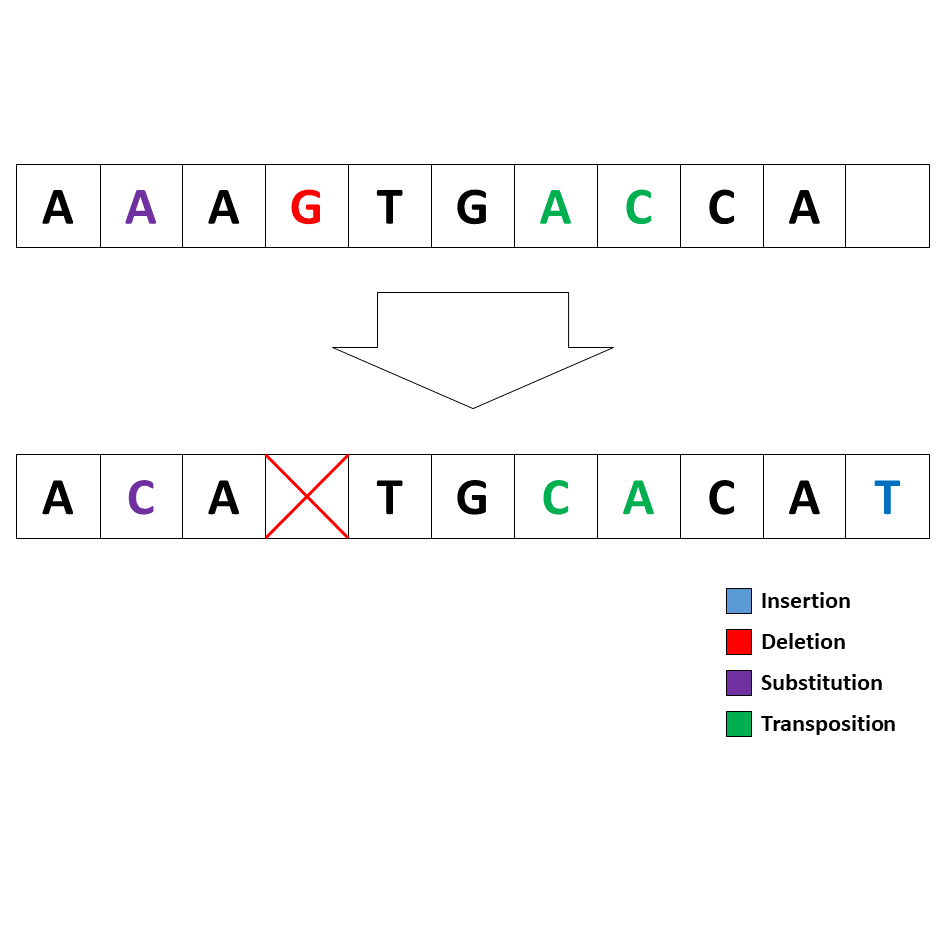
\includegraphics[width=0.75\textwidth]{figures/Graphics/Slide6.PNG}
    \caption{Shows two sequences. The edit distance is the sum of multiple operations. Blue shows an insert, red a deletion, purple a substitution and green a transposition. Therefore the edit distance is 4.}
    \label{fig:dl_example}
\end{figure}


\noindent \autoref{eq:damerau_levenshstein} depicts the recursive formulation of the distance. The distance computes the costs of transforming the sequence $a$ to $b$, by computing the minimum of five seperate terms.  
% TODO: change a to e for consistency with model formulation
% TODO: Read on sequence alignment literature. Also add the readup to the literature review.
\begin{align}
    \label{eq:damerau_levenshstein}
    d_{a, b}(i, j) & =\min
    \begin{cases}
        \editDistance{i-1}{j  }+ 1 & \text { if } i>0                                            \\
        \editDistance{i  }{j-1}+ 1 & \text { if } j>0                                            \\
        \editDistance{i-1}{j-1}+ 1 & \text { if } i, j>0                                         \\
        \editDistance{i-2}{j-2}+ 1 & \text { if } i, j>1 \land a_{i}=b_{j-1} \land a_{i-1}=b_{j} \\
        0                                 & \text { if } i=j=0                                         
    \end{cases}        
\end{align}

\noindent The recursive form $d_{a, b}(i, j)$ for sequences $a$ and $b$ with respective elements $i$ and $j$ takes the minimum of each of each allowed edit operation. In particular, no change, deletion, insertion, substitution and transposition. For each operation, the algorithm adds an edit cost of 1. 


\end{document}